\documentclass{article}
\usepackage[english]{babel}
\usepackage[a4paper,top=2cm,bottom=2cm,left=2.5cm,right=2.5cm,marginparwidth=1.75cm]{geometry} 
\usepackage{hyperref}
\usepackage[authoryear]{natbib}
\usepackage{graphicx}
\usepackage{fancyhdr}
\bibliographystyle{rusnat}

\pagestyle{fancy}
\fancyhf{}
\lhead{Your names}
\rhead{Project Name}
\rfoot{Page \thepage}

\title{Geospatial Data Science: Project Report Template}
\author{Student 1 \& Student 2}
\date{2023-05-12}


\begin{document}

\maketitle

\begin{abstract}
Optional: include an abstract in the beginning of your project report. Suggested abstract structure: 1-2 sentences basic introduction into field. 2-3 sentences more detailed background. 1 sentence clearly stating the general problem being addressed by this particular study. 1 sentence summarizing the main result (“here we show”). 2-3 sentences explaining what the main result reveals/adds. 1-2 sentences to put results into more general context. Optional - if accessibility is enhanced by this: 2-3 sentences to provide broader perspective. Annotated best practice example (from Nature): \url{http://www.cbs.umn.edu/sites/default/files/public/downloads/Annotated_Nature_abstract.pdf}
\end{abstract}

\section*{Technicalities}
\subsection*{Layout}
\begin{itemize}
	\item font size: 11pt
	\item linespacing: single
	\item pages (without references and appendices): 6-10 for a group of 1; 8-12 for a group of 2; 10-14 for a group of 3
	\item must contain at least one figure with geospatial data visualization
\item all tables and figures labelled
\item Collaboration – e.g. on overleaf: \url{ https://www.overleaf.com/}
\end{itemize}
\subsection*{Code repository}
If your project is a prototype of a digital product, don’t hand in the code – instead, include in the report:
\begin{itemize}
	\item a link to your code repository 
	\item an URL (or another way) where your prototype can be tried out
\end{itemize}
If your project is based on a research question, hand in:
\begin{itemize}
\item gitlog.txt: Your repo’s git log, e.g. by running: \texttt{git log > gitlog.txt}
 	\item code.zip: One zip file containing Jupyter notebook(s) (.ipynb) of your commented code that runs fully without errors, assuming that all used data files are in place, and reproduces your findings. Do not include the data files here
\end{itemize}

\section{Introduction}
Here you provide the context and motivation for the problem. What are your research questions, or what does your prototype intend to do/solve? Explain the particular spatial problem you are tackling and its relevance. 

\section{Background}
Provide \textbf{context} (historical, cultural, technical) for your project and introduce the background and related work in literature (cite or list relevant literature on the research problem; list other scripts and software in this area etc.)
Give an overview of the (cultural, historical, social, technical, etc.) problems to be solved by the project and the role of the different digital tools in achieving the aims of the project
Specify your approach and why you have chosen it.

\section{Data}
\subsection{Data acquisition}
List and cite all sources of data used in this paper, comment on their fitness for purpose (format, quality, and provenance). Focus on the spatial component of your data, its origin, and precision and reliability. 

\subsection{Data processing}
Provide details of data manipulation and transformation. Name challenges, if any. Link to processing scripts where relevant.

\section{Results}
Provide and explain the results of your investigation, illustrated with figures where essential and relevant (unlike figure \ref{fig01}). Relate to lessons learnt, counts, statistics, maps or other outcomes.
Briefly comment on 1) the main elements of your digital workflow, highlighting challenges and decision-making bottlenecks (e.g. how did you transform point data to make it into a continuous surface?) 2) functions/tricks you found useful and wish to promote or credit. Remember that the technical tasks should not clutter/interfere with your overall narrative and data analysis (unless your project is about developing a technical pipeline) 
For 'technical pipeline' projects: provide a guided tour of your pipeline to facilitate its reproducibility, explaining your choices, clarifying dependencies, and referring to the scripts/tools you compiled in GitHub.

\begin{figure}[t]
    \centering
    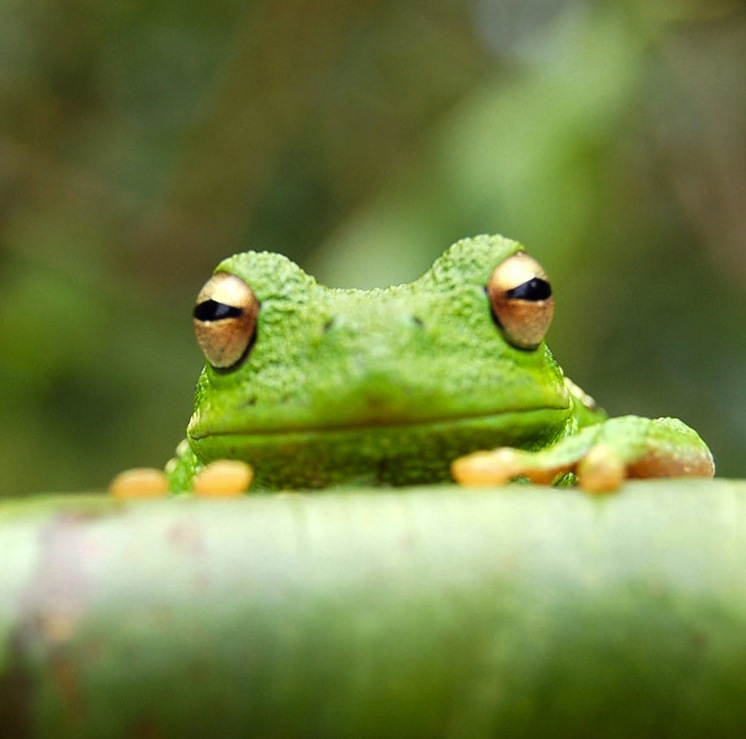
\includegraphics[width=0.3\textwidth]{frog.jpg}
    \caption{A completely unrelated frog.}
    \label{fig01}
\end{figure}

\section{Discussion}
Evaluate the results in light of the data sources and research premises/assumptions. How representative, reliable, complete and precise are your results? How transferable or generalizable? Give an account on the major short-coming(s) of your methodology / data / prototype. Briefly evaluate the results in light of digital tools, the learning process, time on task, vis-à-vis the final product.

\section{Conclusion}
Here you provide a short summary of the results of the project, the achieved (or missed) goals and highlight the most important lessons learnt while working on the project. Indicate how the methods, data, analysis, or prototype functionalities could be improved or extended in future work.

\section{References}
At least 5, both domain-based literature and references to digital tutorials or internet resources consulted. Choose whichever reference system you like - and stick to it. Cite some authors like \cite{greenwade93} - again, you're free to pick any format as long as it's coherent.
Examples:

\begin{itemize}

\item \texttt{\href{https://www.chicagomanualofstyle.org/tools\_citationguide.html}{Chicago Style}}
\item \texttt{\href{https://www.mendeley.com/guides/apa-citation-guide/}{APA}}
\item \texttt{\href{https://www.mendeley.com/guides/harvard-citation-guide/}{Harvard}}

\end{itemize}

\bibliography{sample}

\section*{Appendix A: Meta data tables}

Metadata tables – see project report for details

\section*{Appendix B: Contribution statement}

For individualized grading, you must provide a contribution statement in which you clarify who of your group is responsible for the different parts of the project submission. Please state:

\begin{itemize}
    \item For \textbf{at least 2 sections} of your report, who was \textbf{primary contributor} (and optionally also second and/or third contributor)
    \item For any \textbf{additional major tasks} such as data collection, data preparation, analysis, programming, or visualization, who was \textbf{primary contributor} (optionally also second and/or third contributor)  
\end{itemize}

\end{document}